\section{Graphical User Interface}
In this section, we will present and describe the wireframes of the application. These wireframes illustrate the layout and structure of the user interface across different parts of the system, providing a visual representation of how users will interact with the application. Each wireframe focuses on a specific microfrontend or application shell, showcasing its core functionality and design elements.
\subsection{Application Shell}
\begin{figure}[h]
\centerline{
\includegraphics[width=1\textwidth]{images/wireframes/shell.png}}
\caption[Application shell wireframe]{Application shell wireframe}
\label{shell:wireframe}
\end{figure}
The application shell design features a side panel that contains the logo, standard navigation links for each microfrontend, and a settings button. The main content area next to the side panel serves as the placeholder where microfrontends will be dynamically rendered based on the user's navigation. When the user clicks the settings button, a modal window opens, allowing them to switch languages and toggle between light and dark themes. To keep the document concise, the wireframe for the settings modal is not included, as it would take up additional space.

\subsection{Users Microfrontend}
\begin{figure}[h]
\centerline{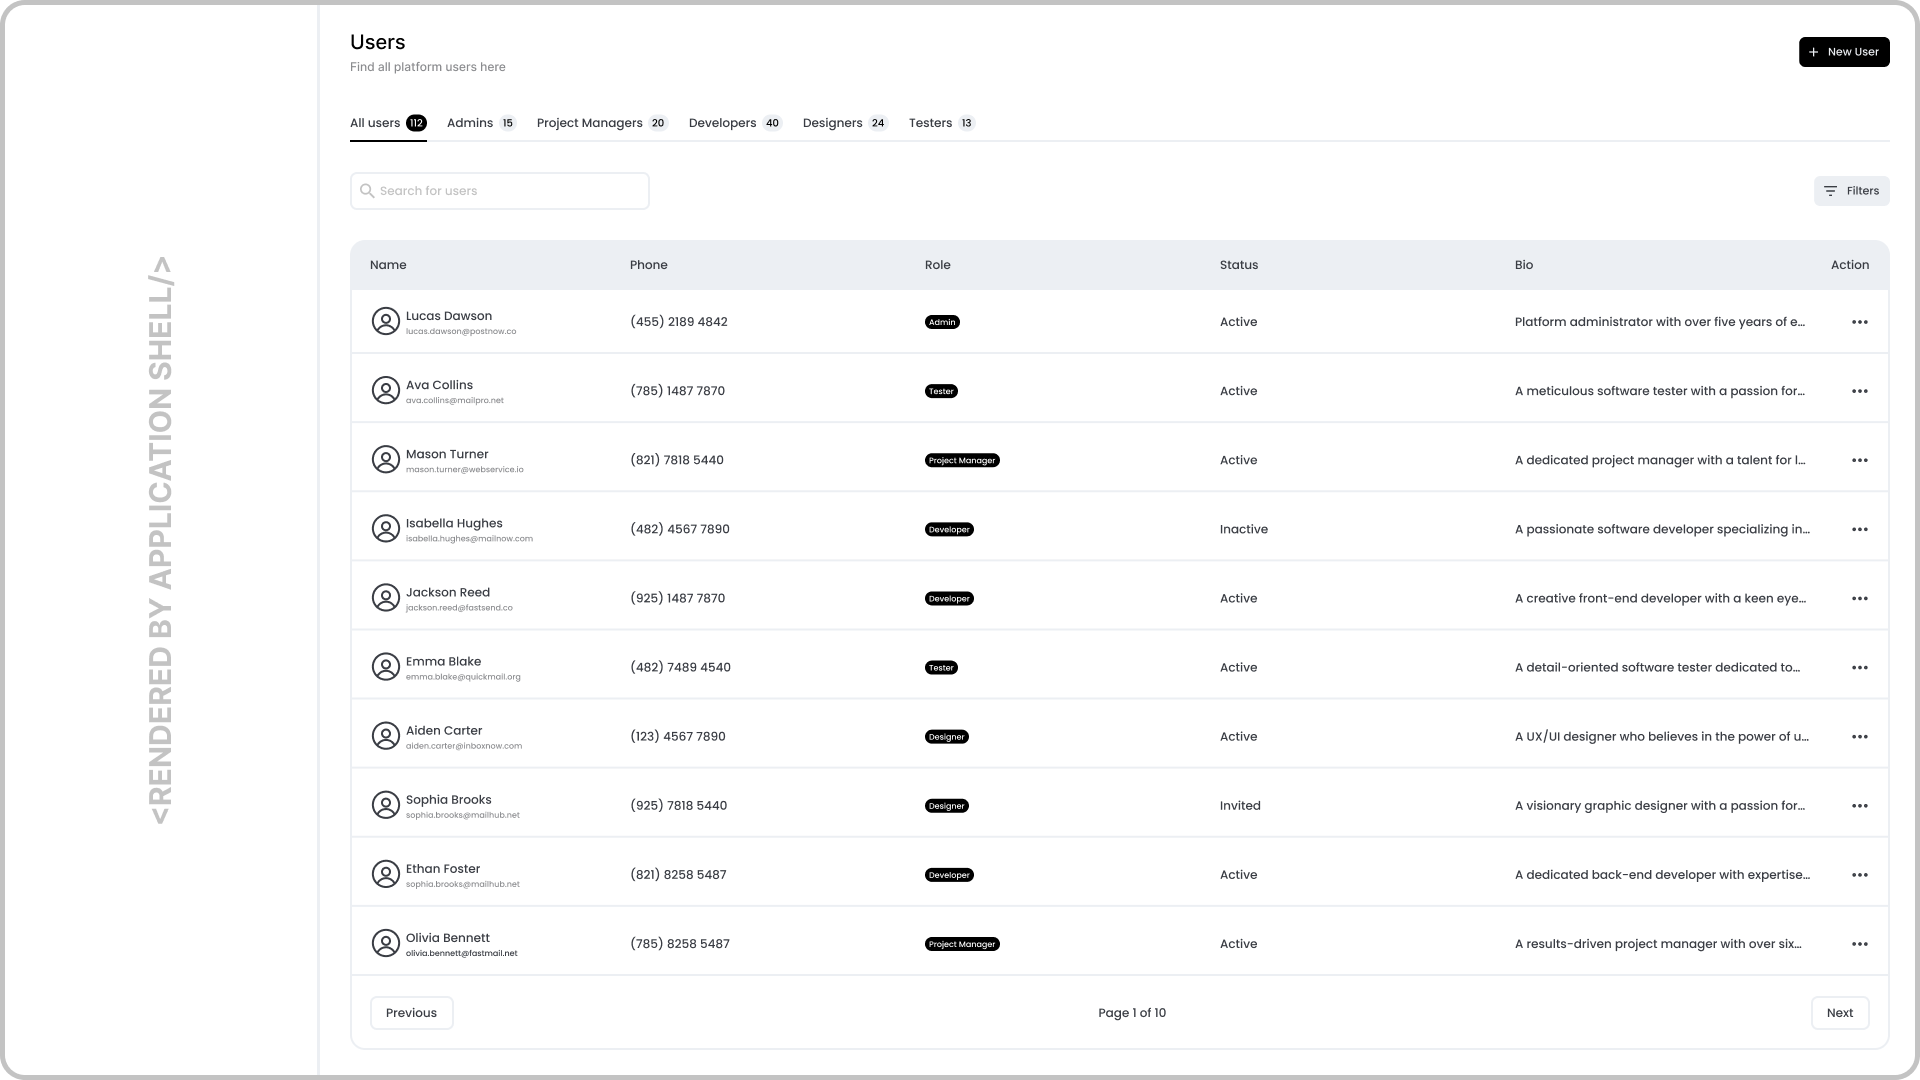
\includegraphics[width=1\textwidth]{images/wireframes/users.png}}
\caption[Users microfrontend wireframe]{Users microfrontend wireframe}
\label{mf:users}
\end{figure}
The Users Microfrontend consists of a table where each row represents a user, displaying key details such as name, email, and role. The last column of the table is dedicated to an action button, which opens a dropdown menu with options to view, edit, or delete a user. Upon selecting any of these actions, a modal window appears, allowing users to execute the desired operation. As with other modals in the application, they are not included in this document to conserve space. Directly above the table is a search bar and a filter button, enabling users to refine the displayed records further. Additionally, a set of tabs allows for quick filtering of users based on their roles (e.g., Admin, Developer, Tester). At the very top, the topbar includes the page title, a brief subtitle, and a button to add a new user. Clicking this button also opens a modal specifically designed for user creation.

\subsection{Projects Microfrontend}
\begin{figure}[h]
\centerline{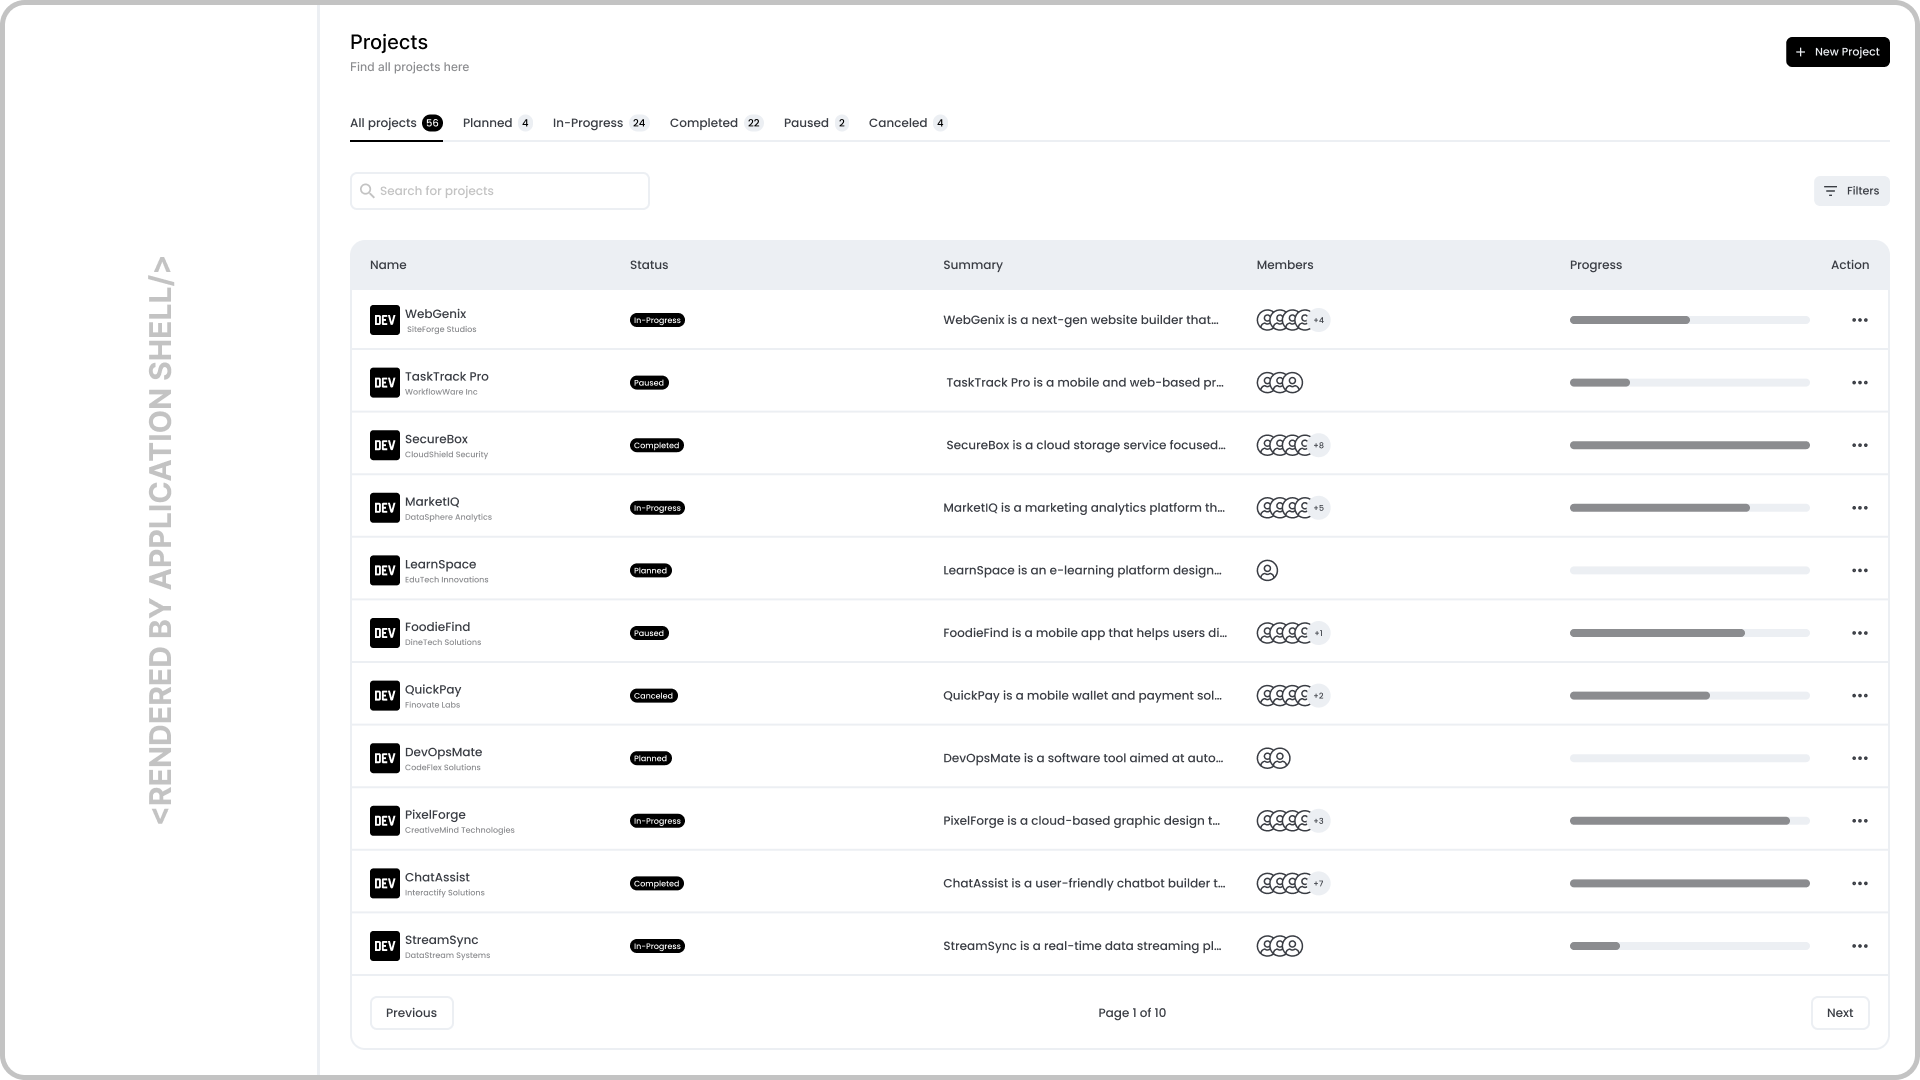
\includegraphics[width=1\textwidth]{images/wireframes/projects.png}}
\caption[Projects microfrontend wireframe]{Projects microfrontend wireframe}
\label{mf:projects}
\end{figure}
The projects microfrontend follows a similar structure to the users microfrontend. It features a table where each row represents a project, displaying key details such as project name, associated company, tags, and other relevant information. The last column of the table is reserved for an action button, which opens a dropdown menu with options to view, edit, or delete the project. Above the table, there is a search bar and a filter button to help users further refine the list of projects. Additionally, a set of tabs allows for quick filtering of projects based on their status (e.g., Planned, In-Progress, Completed), enabling users to quickly locate projects in different stages of development. At the top of the page, the topbar displays the page title, a brief subtitle, and a button to add a new project. Similar to the user management interface, clicking the "Add Project" button opens a modal designed for creating a new project.

\subsection{Tasks Microfrontend}
\begin{figure}[h]
\centerline{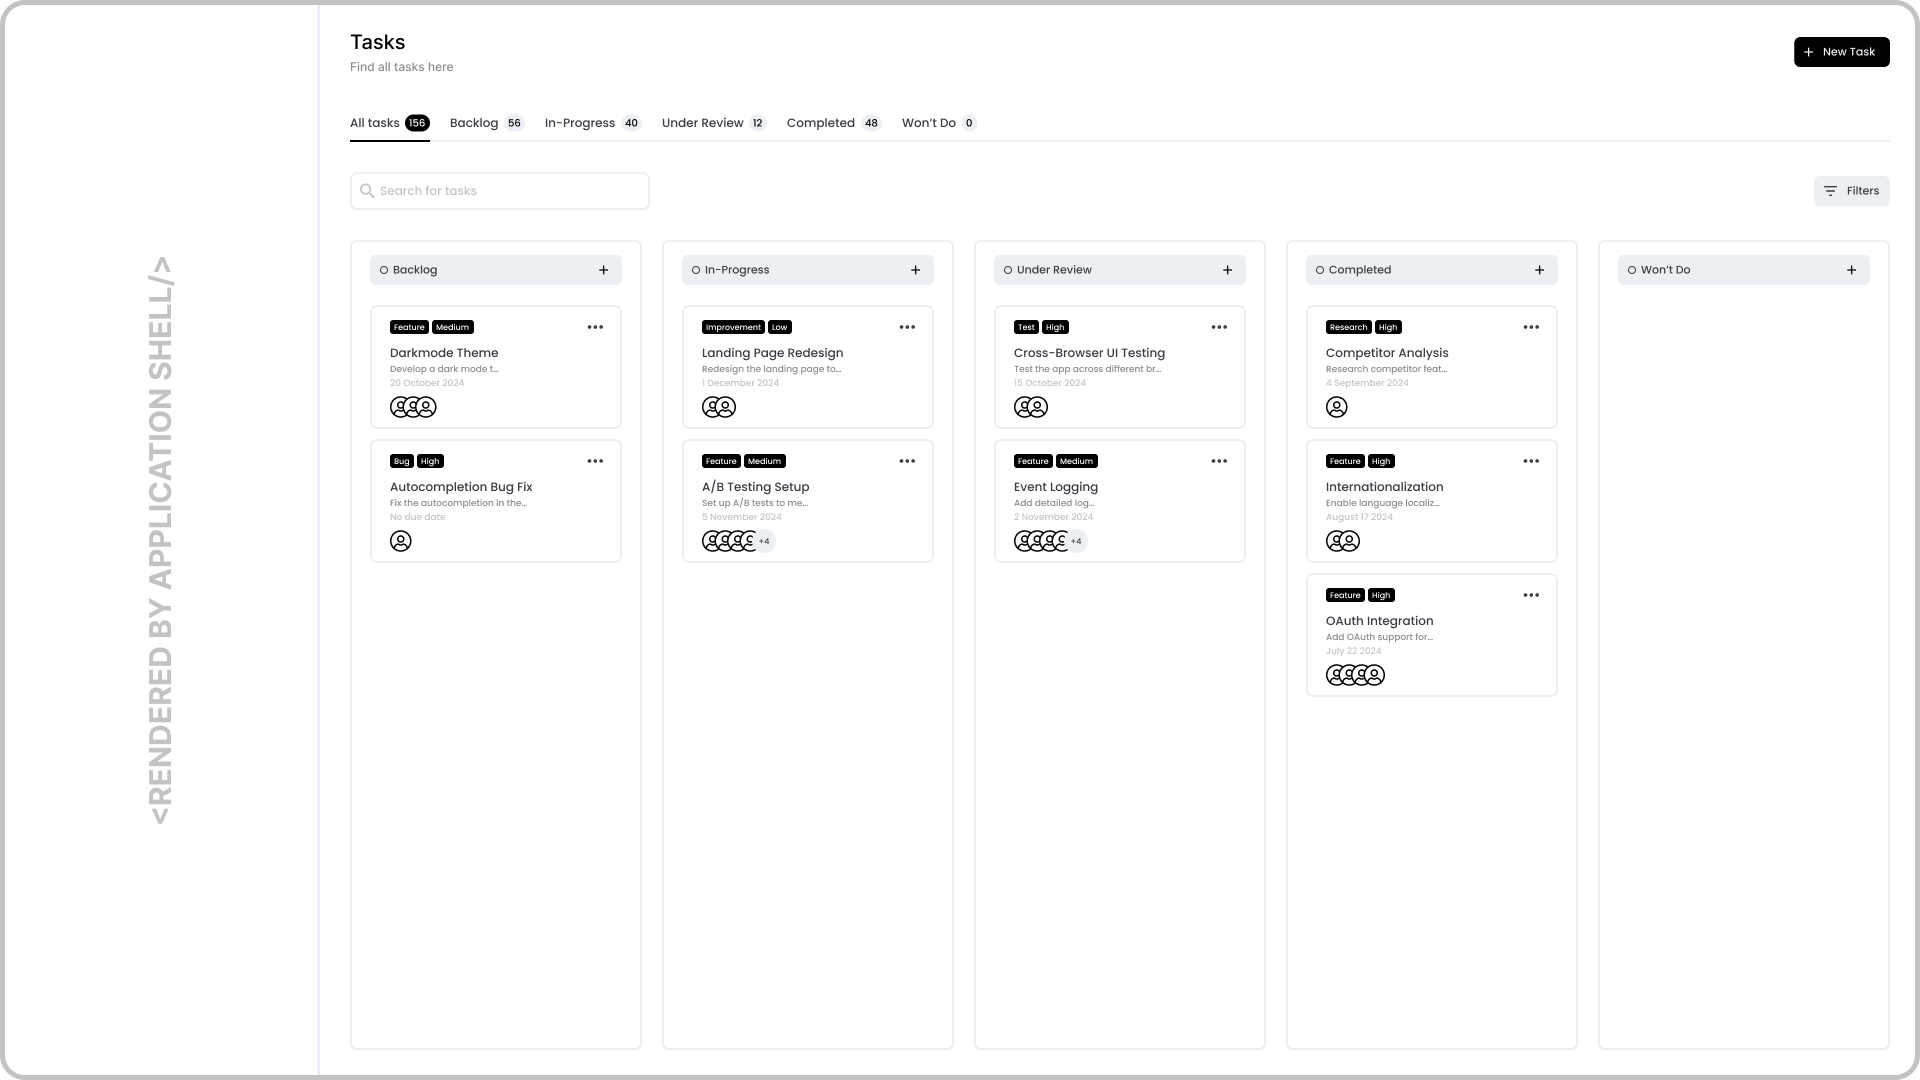
\includegraphics[width=1\textwidth]{images/wireframes/tasks.png}}
\caption[Tasks microfrontend wireframe]{Tasks microfrontend wireframe}
\label{mf:tasks}
\end{figure}
The Tasks Microfrontend is slightly different from the other sections, as its main component is a Kanban board that organizes tasks into various stages, such as Backlog, In-Progress, and Under Review. Each task is represented by a card that displays essential details such as the task title, tags, assignees, and more. In the upper-right corner of each task card, there is a three-dot button that opens a dropdown menu with options to view, edit, or delete the task. Each stage on the Kanban board includes a button for creating new tasks directly within that stage. Above the Kanban board, there is a search bar and a filter button to help users refine the displayed tasks. Additionally, a set of tabs allows for quick filtering of tasks based on their current status, helping users focus on tasks that are relevant to their needs at the moment. At the top of the page, the topbar contains the page title, a brief subtitle, and a button to add a new task. As with other parts of the application, clicking this button opens a modal designed specifically for task creation.

\subsection{Dashboard Microfrontend}
\begin{figure}[h]
\centerline{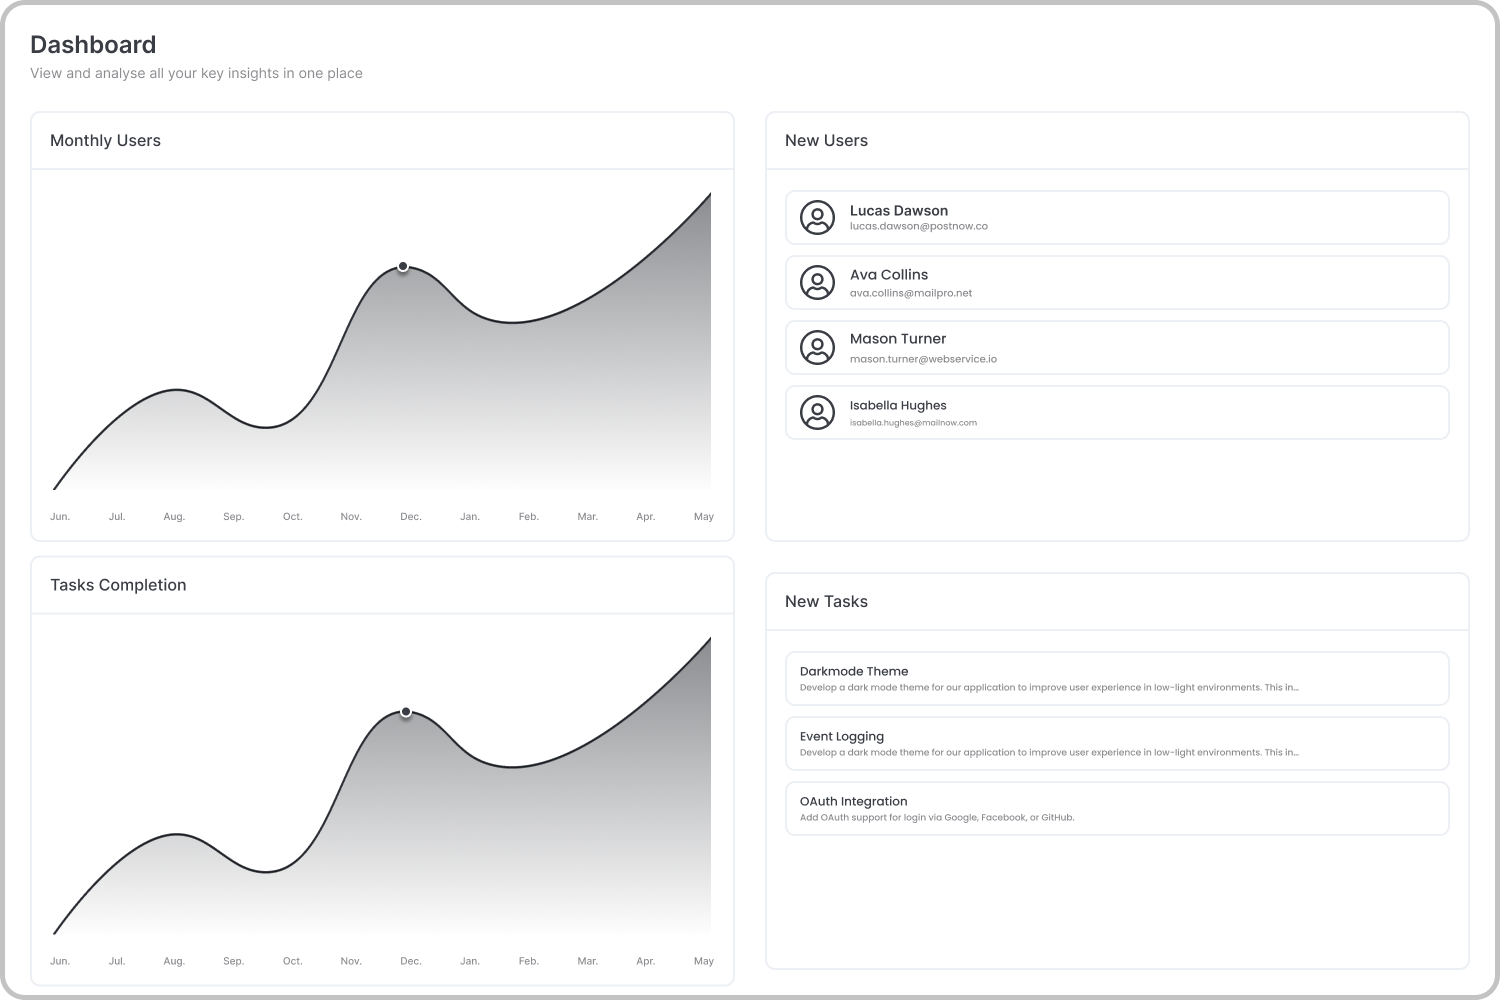
\includegraphics[width=1\textwidth]{images/wireframes/dashboard.png}}
\caption[Dashboard microfrontend wireframe]{ashboard microfrontend wireframe}
\label{mf:dashboard}
\end{figure}
The Dashboard microfrontend provides an overview of key metrics and insights for the current user. At the top of the dashboard, there is a row of summary cards displaying quick statistics for the past month, compared to the previous month. These metrics include: number of active projects, number of new projects, number of completed projects, total number of active tasks, number of new tasks, number of completed tasks. Below this summary, a task completion graph visually represents the number of tasks completed each day over the last month. This graph allows users to track productivity trends at a glance. To the right of the graph is a list of today's tasks, providing a convenient view of tasks assigned to the user that are due or in progress for the current day. Underneath the graph is a list of new members, showing users who have recently joined the system. To the right of this section is a list of the user's projects, displaying each project and its current progress, allowing users to quickly assess the status of their ongoing work.